\documentclass[varwidth=true, border=2pt]{standalone}

\usepackage{pgfplots}
\usepackage{tikz}

\usetikzlibrary{calc,patterns,angles,quotes}

\begin{document}

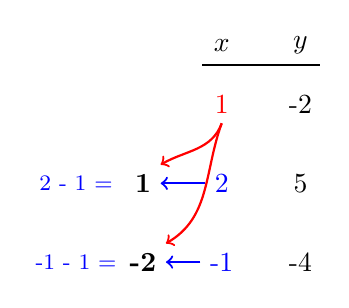
\begin{tikzpicture}
	\node (A) at (1.5,3.25) {$x$};
	\node  (B) [red] at (1.5,2.5){1}; 
	\node (C) [blue] at (1.5,1.5) {2};
	\node (D)[blue] at (1.5,0.5) {-1};
	\node (E) at (0.5,1.5) {\textbf{1}};
	\node (F)  at (0.5,0.5) {\textbf{-2}};
	\node (a) at (2.5,3.25) {$y$};
	\node (b) at (2.5,2.5) {-2};
	\node (c) at (2.5,1.5) {5};
	\node (d) at (2.5,0.5) {-4};

	\draw [->, thick, blue] (C) edge (E) (D) edge (F);
	\draw [->, thick, red] (B.south) to [out=250, in = 30] (E.north east);
	\draw [->, thick, red] (B.south) to  [out=250, in = 30] (F.north east);
	\draw [thick, black] (1.25,3) to (2.75,3);


\footnotesize

	\node [blue] (L1) at (-0.35,0.5) {-1 - 1 =};
	\node [blue]  (L2) at (-0.35,1.5) {2 - 1 =};

\normalsize

\end{tikzpicture}
\end{document}